
\chapter*{Quantum computers and mapping of quantum circuits}
\label{sec:org4b1517f}

\section*{Quantum computing}
\label{sec:org8261f80}

[Intro to Quantum Computation power that it is based on \textbf{superposition} and *entanglement*]
In this section \ldots{}

\subsection*{Essential elements of quantum computation}
\label{sec:org9577ffe}

Qubits and quantum gates are the basic ingredients in quantum computation theory.
As in classical computation with boolean gates and bits, quantum gates operate on the qubits to change their state and return the desired result or calculation.

\begin{itemize}
\item Qubits
\label{sec:org70d95ca}

Qubit stands for quantum bit.
A basic unit of information founded on quantum physics laws.
Unlike a classical bit, whose state can be either \texttt{0} or \texttt{1}, but like a particle; qubits are not in a fixed state -- ground or excited -- until they are measured.
A qubit's state could be either \texttt{0} or \texttt{1} or both before measuring it.
Both ground or excited states are represented in the Dirac's bra-ket notation, viz. \(| 0 \rangle\) and \(| 1 \rangle\) respectively.
This notation holds the algebraic axioms \cite{Nielsen_2009} required to understand the quantum theory.
Prior to measurement, a qubit is described as in a probabilistic state \(| \psi \rangle = \alpha | 0 \rangle + \beta | 1 \rangle\), where \(\alpha, \beta \in \mathbb{C}\) are the so-called probability amplitudes.
\(|\alpha|^2\) is the probability of measuring \(| 0 \rangle\), \(|\beta|^2\) is the probability of measuring \(| 1 \rangle\) and both \(\alpha\) and \(\beta\) are allowed to be complex.
Dirac's notation grants the definition of the quantum states as vectors, as in eq. \ref{eq:org0d14529}.
Moreover, as we will see below, adopting Dirac's axioms will make the quantum theory accessible with classical algebra operations. 

\begin{equation}
\label{eq:org0d14529}
|\psi\rangle = \begin{bmatrix}\alpha \\ \beta \end{bmatrix}
\end{equation}

\textbf{Superposition} is easily described giving values to both \(\alpha\) and \(\beta\) in the same vector.
But, as soon as they are energy probabilistic states, their values are constrained to \(|\alpha|^2 + |\beta|^2 = 1\).
Since quantum states can be described as vectors, one can easily see that the state of a qubit is defined by a 2-dimensional, complex and unitarian vector space.
A \textbf{Hilbert space} \(\mathscr{H}\).
E.g. in eq. \ref{eq:org74f6187} the vectors of the ground, excited and the plus superposition -- a quantum state with the same probability to measure either \(|0\rangle\) or \(|1\rangle\) -- states are depicted, respectively.

\begin{equation}
\label{eq:org74f6187}
|0\rangle = \begin{bmatrix}1 \\ 0 \end{bmatrix} \quad \quad |1\rangle = \begin{bmatrix}0 \\ 1 \end{bmatrix} \quad \quad |+\rangle = \frac{1}{\sqrt{2}} \begin{bmatrix}1 \\ 1 \end{bmatrix}
\end{equation}

As soon as the vectors are 2-dimensional, complex and unitary they can also be described in phase notation (eq. \ref{eq:org3c7b5ea}).
Like the complex numbers, although requiring two angles in this case.
This notation lead us to a very understandable way to visualize the quantum states, the \textbf{Bloch sphere} (fig. \ref{fig:bloch_sphere}).
A sphere of radius one which z-axis extremes represent the ground and excited states.

\begin{equation}
\label{eq:org3c7b5ea}
|\psi \rangle =\cos \left(\theta /2\right)|0\rangle \,+\,e^{i\phi }\sin \left(\theta /2\right)|1\rangle
\end{equation}

\begin{figure}
\centering
\begin{tikzpicture}[line cap=round, line join=round, >=Triangle]
  \clip(-2.19,-2.49) rectangle (2.66,2.58);
  \draw [shift={(0,0)}, lightgray, fill, fill opacity=0.1] (0,0) -- (56.7:0.4) arc (56.7:90.:0.4) -- cycle;
  \draw [shift={(0,0)}, lightgray, fill, fill opacity=0.1] (0,0) -- (-135.7:0.4) arc (-135.7:-33.2:0.4) -- cycle;
  \draw(0,0) circle (2cm);
  \draw [rotate around={0.:(0.,0.)},dash pattern=on 3pt off 3pt] (0,0) ellipse (2cm and 0.9cm);
  \draw (0,0)-- (0.70,1.07);
  \draw [->] (0,0) -- (0,2);
  \draw [->] (0,0) -- (-0.81,-0.79);
  \draw [->] (0,0) -- (2,0);
  \draw [dotted] (0.7,1)-- (0.7,-0.46);
  \draw [dotted] (0,0)-- (0.7,-0.46);
  \draw (-0.08,-0.3) node[anchor=north west] {$\varphi$};
  \draw (0.01,0.9) node[anchor=north west] {$\theta$};
  \draw (-1.01,-0.72) node[anchor=north west] {$\mathbf {\hat{x}}$};
  \draw (2.07,0.3) node[anchor=north west] {$\mathbf {\hat{y}}$};
  \draw (-0.5,2.6) node[anchor=north west] {$\mathbf {\hat{z}=|0\rangle}$};
  \draw (-0.4,-2) node[anchor=north west] {$-\mathbf {\hat{z}=|1\rangle}$};
  \draw (0.4,1.65) node[anchor=north west] {$|\psi\rangle$};
  \scriptsize
  \draw [fill] (0,0) circle (1.5pt);
  \draw [fill] (0.7,1.1) circle (0.5pt);
\end{tikzpicture}
\caption{The Bloch sphere}
\label{fig:bloch_sphere}
\end{figure}

But a system with just one qubit is not useful.
The power of quantum computers explodes with the number of qubits able to work with or, what is the same, the dimensions of the Hilbert space \(\mathscr{H}\).
The quantum state of \(n\) qubits can be represented in bra-ket notation, with a \(2^n\) size.
And, therefore, they engender a Hilbert space of \(2^n\) dimensions due to superposition.
The linear operator that leads to the multiple qubit's state is the \textbf{outer product}, defined as the matrix convolution of the state vectors.
The outer product is represented as \(|\phi \rangle \,\langle \psi |\).
In eq. \ref{eq:org1d1a1dc} and \ref{eq:orgcbdacc7} an example of the outer product is offered.
The second example represents the other main phenomenon in quantum physics, the \textbf{entanglement} state of two qubits (\(\phi\) and \(\psi\)) also known as the Bell state or the Einstein-Podolsky-Rosen (EPR) pair.
\begin{equation}
\label{eq:org1d1a1dc}
|+\rangle \,\langle + | = \frac{1}{\sqrt{4}} \left( \begin{bmatrix}1 \\ 1 \end{bmatrix} \otimes \begin{bmatrix}1 \\ 1 \end{bmatrix} \right) = \frac{1}{\sqrt{4}} \begin{bmatrix}1 \\ 1 \\ 1 \\ 1\end{bmatrix} 
\end{equation}

\begin{equation}
\label{eq:orgcbdacc7}
|\Phi ^{+}\rangle =\frac  {1}{\sqrt  {2}}(|0\rangle _{\phi}\otimes |0\rangle _{\psi}+|1\rangle _{\phi}\otimes |1\rangle _{\psi}) =  \frac{(|00\rangle +|11\rangle )} {\sqrt {2}}
\end{equation}


\item Quantum Operations
\label{sec:org0d3e284}

Quantum operations leverage the power of quantum computers enabling calculations over the qubits.
Or what is the same, enabling transformations of a Hilbert space.
One can find a parallelism with the classical computation fundamental operations, the logical operations.
As their classical siblings, the quantum operations are usually represented as gates in a circuit, a so-called quantum circuit.
Quantum operations can be described in Dirac's notation as well.
They are represented as square matrices of \(2^{n} \times 2^{n}\), where \(n\) is the number of qubits involved in the operation.
This matrices should be unitary respecting the qubit state vector unitary property (\(|\alpha|^2 + |\beta|^2 = 1\)).
They shouldn't ever change the amplitude of the state.
Therefore, quantum operations are, basically, state rotations in the Bloch sphere (fig. \ref{fig:bloch_sphere}).
Although, while implying multiple qubits, the quantum operations are more complex than just rotations, as it will be seen below.
For instance, a rotation of 180° in x-axis of the Bloch sphere is the same as an operation that changes the qubit state from \(| 0 \rangle\) to \(| 1 \rangle\), or viceversa.
Qubits and quantum operations interact through the \textbf{inner product}.
In order to apply some operation over a qubit state, a matrix-vector multiplication should be done.
For instance, in eq. \ref{eq:org77bbb22} one can understand how some uniform operation \(U\) is applied to a qubit with state \(| \psi \rangle\).

\begin{equation}
\label{eq:org77bbb22}
U |\psi\rangle=\begin{bmatrix}u_{00}&u_{01}\\u_{10}&u_{11}\end{bmatrix} \begin{bmatrix}\alpha \\ \beta \end{bmatrix} = \begin{bmatrix}\alpha u_{00} + \beta u_{01} \\ \alpha u_{10} + \beta u_{11} \end{bmatrix}
\end{equation}

Also comparable with the boolean gates, quantum operations can be decomposed in other set of quantum operations.
\textbf{Universal set of gates} is a set of operations able to generate any other gate by combining them \cite{Nielsen_2009}.
In classical computation, for example, the \texttt{OR} and the \texttt{AND} gates are able to generate any other logic gate.
In quantum computation there are several universal set of gates.
In the \href{chapter-3.org}{Constraints of the Surface-7 and -17 chips} section we offer a table with a universal gate set with its decomposition, particularized for the SC-7 and -17 chips which specifications will be also described in that section.
It is common to differ between single- and multiple-qubit gates, due to the complexity variation between them.
It is generally accepted to analyze the multiple-qubit gate problem in its most elemental case, that is the two-qubit gates.

\begin{itemize}
\item Single-qubit gates
\label{sec:orgbaa2217}

Single qubit gates represent quantum operations that involve just one qubit.
They are represented as a box with one input and one output, evincing that a single qubit will be the input and output of the operation.
As explained before, single-qubit gates can be represented as \(2^1 \times 2^1\) square matrices that should be unitary.
Both representations of the most common single-qubit gates can be found in Table \ref{tab:org0ed8a39}.

\begin{table}[htbp]
\caption{\label{tab:org0ed8a39}
Most common single qubit gates}
\centering
\begin{tabular}{ccccccc}
Identity & Pauli-X & Pauli-Y & Pauli-Z & Hadamard & S gate & T gate\\
\Qcircuit @C=1em @R=.7em {
  \lstick{|q\rangle} & \gate{I} & \qw\\
}
 & \Qcircuit @C=1em @R=.7em {
  \lstick{\shortmid q\rangle} & \gate{I} & \qw\\
}
 & \Qcircuit @C=1em @R=.7em {
  & \gate{Y} & \qw\\
}
 & \Qcircuit @C=1em @R=.7em {
  \lstick{|q\rangle} & \gate{Z} & \qw\\
}
 & \Qcircuit @C=1em @R=.7em {
  & \gate{H} & \qw\\
}
 & \Qcircuit @C=1em @R=.7em {
  \lstick{|q\rangle} & \gate{S} & \qw\\
}
 & \Qcircuit @C=1em @R=.7em {
  \lstick{|q\rangle} & \gate{T} & \qw\\
}
\\
\(\begin{bmatrix}1&0\\0&1\end{bmatrix}\) & \(\begin{bmatrix}0&1\\1&0\end{bmatrix}\) & \(\begin{bmatrix}0&-i\\i&0\end{bmatrix}\) & \(\begin{bmatrix}1&0\\0&-1\end{bmatrix}\) & \(\frac{1}{\sqrt{2}}\begin{bmatrix}1&1\\1&-1\end{bmatrix}\) & \(\begin{bmatrix}1&0\\0&i\end{bmatrix}\) & \(\begin{bmatrix}1&0\\0&e^{i \pi / 4}}\end{bmatrix}\)\\
\end{tabular}
\end{table}

The \emph{Identity} gate is the idling operation.
It is equivalent to no applying any operation for a cycle.
The \emph{Pauli-x, -y and -z} gates are 180° rotation over the x-, y- and z-axis respectively.
Eg. a qubit with state \(|+\rangle\) that is equivalent to the position \(\theta = \frac{\pi}{2}, \phi = 0\) in the Bloch sphere is rotated in the y-axis with a Pauli-y gate, \(Y|+\rangle = \frac{i}{\sqrt{2}} \begin{bmatrix}-1 \\ 1 \end{bmatrix}\).
This resulting state is located in \(\theta = \frac{\pi}{2}, \phi = \pi\), that is a 180° rotation in the Y axis.
The \emph{Hadamard} gate is also a 180° rotation, but over the diagonal axis between the x- and z-axes, \(\frac{({\hat {x}}+{\hat {z}})}{\sqrt {2}}}\).
The \emph{S} and \emph{T} gates are also rotations over the z-axis but of 90° and 45° respectively.


\item Two-qubit gates
\label{sec:org9d08793}

Two-qubit gates are quantum operations that involve two qubits at the same time.
In general, the two-qubit gates execute a single-qubit operation over one of the qubits, depending on the state of the other.
The qubits that goes through the operation is called \textbf{target}, while the other is called the \textbf{control} qubit.
The most common two-qubit gates are represented in Table \ref{tab:orgf1da05b}.
The \emph{CNOT} gate is a Controlled-NOT operation or, what is the same, a Pauli-x gate that, depending on the state of the control qubit will be executed or not.
As the CNOT, the \emph{CZ} gate is a Controlled-Z operations that, in this case, executes a Pauli-z gate depending on the state of the control qubit.
Finally, the \emph{SWAP} gate "swaps" the state of two qubits.
It moves the state of one to the other and viceversa.
This gate is mostly used for routing purposes as it will be seen in the next sections.

\begin{table}[htbp]
\caption{\label{tab:orgf1da05b}
Most common two-qubit gates}
\centering
\begin{tabular}{ccc}
CNOT & CZ & SWAP\\
\Qcircuit @C=1em @R=.7em {
  & \targ & \qw\\
  & \ctrl{-1} & \qw\\
}
 & \Qcircuit @C=1em @R=.9em {
  & \ctrl{1} & \qw\\
 & \control \qw & \qw\\
}
 & \Qcircuit @C=1em @R=.7em {
 & \qswap & \qw\\
  & \qswap \qwx[-1] & \qw\\
}
\\
\(\begin{bmatrix}1&0&0&0\\0&1&0&0\\0&0&0&1\\0&0&1&0\end{bmatrix}\) & \(\begin{bmatrix}1&0&0&0\\0&1&0&0\\0&0&1&0\\0&0&0&-1\end{bmatrix}\) & \(\begin{bmatrix}1&0&0&0\\0&0&1&0\\0&1&0&0\\0&0&0&1\end{bmatrix}\)\\
\end{tabular}
\end{table}
\end{itemize}
\end{itemize}

\subsection*{Quantum Circuits}
\label{sec:org12b1f41}

Quantum circuits are quantum algorithms descriptions.
As mentioned before, they are formed by quantum gates and qubits connected in circuit fashion.
As most of the algorithm description models -- no matter if classical or quantum --, quantum circuits are hardware agnostic, which is that they are not specified to any quantum device.
They are general descriptions of quantum algorithms.
Besides the circuit description model, quantum algorithms are commonly described as instruction languages like QASM (Quantum ASseMbly) \cite{Nielsen_2009} or its related posterior languages -- cQASM, OpenQASM, etc.
In fig. \ref{fig:circuit_example} we present an example of a quantum circuit.
This circuit represents the quantum equivalent of a Gray encoder of six bit length.
It is composed by CNOT gates only.
An example of the Gray code is shown in \ref{fig:gray_code_example} for different number of bits (\(n\)).
Also, the QASM algorithm representation can be seen in Fig. \ref{code:qasm_gray_code}.

\begin{figure}
    \centering

\resizebox{0.2\textwidth}{!}{
   \Qcircuit @C=1em @R=.7em {
\lstick{a} & \targ & \qw & \qw & \qw & \qw & \qw\\
\lstick{b} & \ctrl{-1} & \targ & \qw & \qw & \qw & \qw\\
\lstick{c} & \qw & \ctrl{-1} & \targ & \qw & \qw & \qw\\
\lstick{d} & \qw & \qw & \ctrl{-1} & \targ & \qw & \qw\\
\lstick{e} & \qw & \qw & \qw & \ctrl{-1} & \targ & \qw\\
\lstick{f} & \qw & \qw & \qw & \qw & \ctrl{-1} & \qw
}
}

\label{fig:circuit_example}
\caption{Gray encoder quantum circuit.}
\end{figure}

\begin{figure}[htbp]
\centering
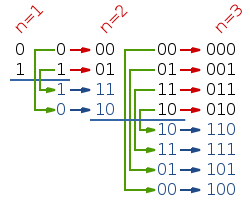
\includegraphics[width=0.3\textwidth]{figures/gray_code.png}
\caption{\label{fig:org120ac4b}
Gray Code example for 3 bits.}
\end{figure}

\begin{figure}
\centering
\begin{minipage}{.45\textwidth}

\begin{minted}[frame=lines,fontsize=\scriptsize,linenos,breaklines,breakanywhere]{c}

#QASM code

# qubit declaration
qubit a
qubit b
qubit c
qubit d
qubit e
qubit f

# gates declaration
cnot b,a
cnot c,b
cnot d,c
cnot e,d
cnot f,d

\end{minted}

\caption{QASM code describing the Gray code algorithm.}
\label{code:qasm_gray_code}
\end{minipage}
\end{figure}

\subsection*{Quantum Error Correction (QEC) and Fault Tolerant (FT) quantum computation}
\label{sec:orgd378c45}
Quantum operations are faulty and qubits are not able to hold the desired state for long times, gradually rotating to another state -- the qubit decoheres.
For instance, in the case of superconducting technologies \cite{O_Brien_2017}, the chips bear with decoherence times of \(\approx 30 \mu s\) for qubit relaxation and \(\approx 60 \mu s\) for qubit dephase.
The error rates of single-qubit gates are less than 0.1\% taking \(> 20 ns\) to be executed, while two-qubit gates error rate is 0.6\% with times of \(40 ns\) and measurement error rates around 1\% with execution times of \(\sim 300 ns\) \cite{O_Brien_2017,Versluis_2017}.
This creates an undesirable environment to compute the most useful algorithms.
Therefore, in order to fight the errors generated by this behaviour, fault-tolerant (FT) and quantum error correction (QEC) mechanisms have been developed during the last years \cite{Nielsen_2009}.

\section*{Mapping of quantum circuits}
\label{sec:org91fa415}

As it was described in the [LINK TO THE SECTION DESCRIBING THE FULL STACK] the mapping step is a critical part of the quantum compilation.
Quantum computers have limitations (\href{chapter-3.org}{Constraints of the Surface-7 and -17 chips}) that are not contemplated in the quantum circuits description due to its inherent hardware agnostic behaviour.
One of the main constraints is the Nearest Neighbor (NN) constraint.
This curb alludes to the qubit connectivity inside the quantum processors, affecting the two-qubit gates realization.
Instead of connected in an all-to-all fashion, the qubits are arranged in a two-dimensional grid shape, connecting each qubit to other four qubits -- its neighbours.
At the same time, the quantum circuits consider the qubits arranged in an all-to-all fashion, applying two-qubit gates to qubits no matter if they are neighbors or not.
Then, the circuits need a transformation in order to be executed in real quantum devices.
The qubits states need to switch places between them -- with SWAP gates -- whenever an interaction between two qubits that are not NN is required. 

The mapping process adapts a quantum circuit representation to the requirements of a real quantum processor.
It brings ideal algorithms down to earth, to the limitations of the quantum chips.
Therefore, the mapping accounts for the realization of quantum algorithms in quantum chips.
As explained in the previous section (\hyperref[sec:orgd378c45]{Quantum Error Correction (QEC) and Fault Tolerant (FT) quantum computation}), quantum gates are faulty.
Then, the extra addition of them due to the mapping task causes quantum algorithms to accumulate error and result in noisy or even useless results.
Therefore, the optimal mapping would be the one that alters the least the original circuit.
In order to address the mapping problem, we split it in three steps, viz.: \textbf{scheduling}, \textbf{initial placement} and \textbf{routing}.
These steps can be executed several times, or even continuously, and in any order, depending on the mapping approach.

\begin{itemize}
\item Initial placement
\label{sec:orgbf3f616}

Throughout this thesis we use the terms \textbf{\emph{virtual} qubits} and \textbf{\emph{physical} qubits} referring to the qubits from the circuit we would like to adapt -- map -- and the real qubits from the quantum chip, respectively.
The initial placement task is responsible to relate the virtual qubits with the physical ones finding the best 
As one can see in the example below, and in more detail in Tab. \ref{tab:org9cd562c}, the initial placement is a crucial part of the optimal mapping.
Depending on its quality, it would make the routing work easier or even make the optimal mapping impossible to find.

\item Routing
\label{sec:org2479518}

The routing process accounts for finding the best path between two qubits far away in the chip layout.
It introduces the SWAP gates -- or a decomposition of it -- to move the qubit states from one point to another.
Therefore, it is a decisive step in order to reduce the number of added gates to the circuit.
Then, the routed best path is the one that introduces the less number of gates to the overall circuit.
It could be the case that the best path for some two-qubit gate would introduce the least number of operations for this operation but it could make the overall circuit bigger.
Eg. let us consider three qubits far away-- \(q_1, q_2, q_3\) -- and two operations, \texttt{CNOT q\_1,q\_2} and \texttt{CNOT q\_1,q\_3}.
The three qubits are far away from each other and \(q_1\) is located between \(q_2\) and \(q_3\).
It could be the case that a mapping algorithm decides that the best path for the first operation is to swap \(q_1\) close to \(q_2\), but that would make the path to \(q_3\) -- the next operation -- longer.
On the contrary, if the mapping algorithm would decide to move \(q_2\) closer to \(q_1\), it would make the overall number of added gates much smaller.
We will appreciate the behaviour of the initial placement and the routing steps as an example in the next subsection (\hyperref[sec:orgefba2ad]{Mapping example}).

\item Scheduling
\label{sec:org3a13e41}

A scheduler organizes the circuit operations through the circuit time,
finding whether several operations can be executed in parallel -- at the same time -- or not.
It is possible to schedule in different configurations, for instance \emph{*As Soon As Possible} (ASAP)* or \emph{*As Late As Possible} (ALAP)*, depending on the mapping requirements.
As an example of scheduling, let's consider the circuit in Fig. \ref{fig:scheduling_ex}
Notice that, in the example, there are several combinations of parallel operations.
Depending on the scheduling configuration,
the operations will be spread along the circuit in one way or the other.

A dependence graph is a graph that relates qubits and gates sequentially.
Starting from the qubits, it chains all the gates with them.
It is really convenient while mapping, mostly scheduling and finding the parallel operations.
Fig. \ref{fig:dependence_graph_ex} shows the dependence graph of the circuit in Fig. \ref{fig:scheduling_ex} as an example.
One can see how the gates that are in the same column --SWAP and CNOT, H and X -- can run in parallel.

\begin{figure}
    \centering

\subfigure[Original circuit]{

%\resizebox{0.3\textwidth}{!}{
\Qcircuit @C=1em @R=.7em {
 & \qswap & \qw & \gate{X} & \qw & \qw\\
 & \qw & \ctrl{2} & \qw & \qw & \qw\\
 & \qswap \qwx[-2] & \qw & \qw & \gate{H} & \qw\\
 & \qw & \targ & \qw & \qw & \qw\\
}
%}
}
\label{fig:scheduling_ex_orig}

\subfigure[ASAP]{

%\resizebox{0.3\textwidth}{!}{
   \Qcircuit @C=1em @R=.7em {
 &  &  & \qwx[5] &  & \\
 & \qswap & \qw & \qw & \gate{X} & \qw\\
 & \qw & \ctrl{2} & \qw & \qw & \qw\\
 & \qswap \qwx[-2] & \qw & \qw & \gate{H} & \qw\\
 & \qw & \targ & \qw & \qw & \qw\\
 &  &  &  &  & \\
}
%}
}
\label{fig:scheduling_ex_asap}

\subfigure[ALAP]{

%\resizebox{0.3\textwidth}{!}{
\Qcircuit @C=1em @R=.7em {
 & \qswap & \qw & \gate{X} & \qw & \qw\\
 & \qw & \ctrl{2} & \qw & \qw & \qw\\
 & \qswap \qwx[-2] & \qw & \qw & \gate{H} & \qw\\
 & \qw & \targ & \qw & \qw & \qw\\
}
%}
}
\label{fig:scheduling_ex_alap}

\caption{Scheduling example}
\label{fig:scheduling_ex}
\end{figure}


\begin{figure}
\centering
\resizebox{.3\textwidth}{!}{%
\begin{tikzpicture}
    
    \node [draw, rectangle] (a) at (0,3) {a};
    \node [draw, rectangle] (b) at (0,2) {b};
    \node [draw, rectangle] (c) at (0,1) {c};
    \node [draw, rectangle] (d) at (0,0) {d};

    
    \node [draw, ellipse] (swap) at (2,2) {SWAP};
    \node [draw, ellipse] (cnot) at (2,1) {CNOT};
    \node [draw, ellipse] (x) at (4,2.5) {X};
    \node [draw, ellipse] (h) at (4,1.5) {H};
   
    
    \draw (a) -- (swap);
    \draw (c) -- (swap);
    
    \draw (b) -- (cnot);
    \draw (d) -- (cnot);
    
    \draw (swap) -- (h);
    
    \draw (swap) -- (x);
    
    
\end{tikzpicture}
}
\caption{Dependence graph of the scheduling example (Fig. \ref{fig:scheduling_ex})}
\label{fig:dependence_graph_ex}
\end{figure}
\end{itemize}

\item Mapping example
\label{sec:orgefba2ad}

\begin{figure}
\centering
\subfigure[Gray code circuit to map]{
\begin{figure}
\Qcircuit @C=1em @R=.7em {
\lstick{a} & \targ & \qw & \qw & \qw & \qw & \qw\\
\lstick{b} & \ctrl{-1} & \targ & \qw & \qw & \qw & \qw\\
\lstick{c} & \qw & \ctrl{-1} & \targ & \qw & \qw & \qw\\
\lstick{d} & \qw & \qw & \ctrl{-1} & \targ & \qw & \qw\\
\lstick{e} & \qw & \qw & \qw & \ctrl{-1} & \targ & \qw\\
\lstick{f} & \qw & \qw & \qw & \qw & \ctrl{-1} & \qw
}
\end{figure}

}
\label{fig:map_ex_circ}

\subfigure[Dependence graph of the circuit]{
\resizebox{\textwidth}{!}{%
\begin{tikzpicture}

%maximum width= pt
    
    \node [draw, rectangle] (a) at (0,5) {a};
    \node [draw, rectangle] (b) at (0,4) {b};
    \node [draw, rectangle] (c) at (0,3) {c};
    \node [draw, rectangle] (d) at (0,2) {d};
    \node [draw, rectangle] (e) at (0,1) {e};
    \node [draw, rectangle] (f) at (0,0) {f};
    
    \node [draw, ellipse] (cnot1) at (2,4.5) {CNOT a,b};
    \node [draw, ellipse] (cnot2) at (4,3.5) {CNOT b,c};
    \node [draw, ellipse] (cnot3) at (6,2.5) {CNOT c,d};
    \node [draw, ellipse] (cnot4) at (8,1.5) {CNOT d,e};
    \node [draw, ellipse] (cnot5) at (10,0.5) {CNOT e,f};


    \draw (a) -- (cnot1);
    \draw (b) -- (cnot1);
    
    \draw (cnot1) -- (cnot2);
    \draw (c) -- (cnot2);
    
    \draw (cnot2) -- (cnot3);
    \draw (d) -- (cnot3);
    
    \draw (cnot3) -- (cnot4);
    \draw (e) -- (cnot4);
    
    \draw (cnot4) -- (cnot5);
    \draw (f) -- (cnot5);
    
\end{tikzpicture}
}
Latency: 400ns

}
\label{fig:map_ex_depend}

\subfigure[Chip layout where to map the example circuit]{
\resizebox{0.45\textwidth}{!}{%
     \begin{tikzpicture}[x=5mm,y=5mm]
 % \tikzstyle{every node} = [circle, fill=gray!30]
 % \node [green] at (0,0) {[circle, fill=gray!30]};
 \draw node[fill=cyan,circle,minimum size=0.3cm] at (0,0) {};
 % \node [cyan] at (10,0) {\textbullet};
 \draw node[fill=cyan,circle,minimum size=0.3cm] at (10,0) {};
 % \node [green] at (20,0) {\textbullet};
 \draw node[fill=cyan,circle,minimum size=0.3cm] at (20,0) {};
 % \node [red] at (5,5) {\textbullet};
 \draw node[fill=cyan,circle,minimum size=0.3cm] at (5,5) {};
 % \node [red] at (5,-5) {\textbullet};
 \draw node[fill=cyan,circle,minimum size=0.3cm] at (5,-5) {};
 % \node [red] at (15,5) {\textbullet};
 \draw node[fill=cyan,circle,minimum size=0.3cm] at (15,5) {};
 % \node [red] at (15,-5) {\textbullet};
 \draw node[fill=cyan,circle,minimum size=0.3cm] at (15,-5) {};

 \node [purple] at (1,0) {\textbf{2}};
 \node [purple] at (11,0) {\textbf{3}};
 \node [purple] at (21,0) {\textbf{4}};
 \node [purple] at (6,5) {\textbf{0}};
 \node [purple] at (6,-5) {\textbf{5}};
 \node [purple] at (16,5) {\textbf{1}};
 \node [purple] at (16,-5) {\textbf{6}};

 % \draw[{Circle[red]}-Latex] (0,0) -- (2,0);
 \draw[-Latex] (0.1, 0.4)  -- (4.6,4.9);
 %% \draw[-Latex] (0.1, 0.4)  -- (4.6,4.9)   node [midway, above, sloped] {0};
 %% \draw[-Latex] (4.8,4.7)   -- (0.3,0.2)  node [midway, below, sloped] {8};

 \draw[-Latex] (5.4, 4.9)   -- (9.9,0.4);
 %% \draw[-Latex] (5.4, 4.9)   -- (9.9,0.4)  node [midway, above, sloped] {1};
 %% \draw[-Latex] (9.7,0.2) -- (5.2,4.7)   node [midway, below, sloped] {9};

 \draw[-Latex] (10.1,0.4)  -- (14.6,4.9);
 %% \draw[-Latex] (10.1,0.4)  -- (14.6,4.9)  node [midway, above, sloped] {2};
 %% \draw[-Latex] (14.8,4.7)  -- (10.3,0.2) node [midway, below, sloped] {10};

 \draw[-Latex] (15.4, 4.9)  -- (19.9,0.4);
 %% \draw[-Latex] (15.4, 4.9)  -- (19.9,0.4)  node [midway, above, sloped] {3};
 %% \draw[-Latex] (19.7,0.2) -- (15.2,4.7)  node [midway, below, sloped] {11};

 \draw[-Latex] (0.4,-0.1) -- (4.9,-4.6);
 %% \draw[-Latex] (0.4,-0.1) -- (4.9,-4.6)  node [midway, above, sloped] {4};
 %% \draw[-Latex] (4.7,-4.8) -- (0.2,-0.3)  node [midway, below, sloped] {12};

 \draw[-Latex] (5.1, -4.6) -- (9.6,-0.1);
 %% \draw[-Latex] (5.1, -4.6) -- (9.6,-0.1) node [midway, above, sloped] {5};
 %% \draw[-Latex] (9.8, -0.3) -- (5.3, -4.8) node [midway, below, sloped] {13};

 \draw[-Latex] (10.4,-0.1) -- (14.9,-4.6);
 %% \draw[-Latex] (10.4,-0.1) -- (14.9,-4.6) node [midway, above, sloped] {6};
 %% \draw[-Latex] (14.7,-4.8) -- (10.2,-0.3) node [midway, below, sloped] {14};

 \draw[-Latex] (15.1,-4.6) -- (19.6,-0.1);
 %% \draw[-Latex] (15.1,-4.6) -- (19.6,-0.1) node [midway, above, sloped] {7};
 %% \draw[-Latex] (19.8,-0.3)  -- (15.3,-4.8) node [midway, below, sloped] {15};

 \end{tikzpicture}
 }

}
\label{fig:map_ex_chip}

\label{fig:map_ex_def}
\caption{Mapping example draft}
\end{figure}

\begin{figure}
\centering
\subfigure[Qubits initialization in a naive way]{
\Qcircuit @C=1em @R=.7em {
     \lstick{a \to Q_0} & \targ & \qw & \qw & \qw & \qw & \qw\\
\lstick{b \to Q_2} & \ctrl{-1} & \targ & \qw & \qw & \qw & \qw\\
\lstick{c \to Q_5} & \qw & \ctrl{-1} & \targ & \qw & \qw & \qw\\
\lstick{d \to Q_3} & \qw & \qw & \ctrl{-1} & \targ & \qw & \qw\\
\lstick{e \to Q_1} & \qw & \qw & \qw & \ctrl{-1} & \targ & \qw\\
\lstick{f \to Q_4} & \qw & \qw & \qw & \qw & \ctrl{-1} & \qw
}

}
\label{fig:map_ex_circ_wrong}

\subfigure[Qubit disposition in the chip layout]{
\resizebox{0.4\textwidth}{!}{%
     \begin{tikzpicture}[x=5mm,y=5mm]
 % \tikzstyle{every node} = [circle, fill=gray!30]
 % \node [green] at (0,0) {[circle, fill=gray!30]};
 \draw node[fill=cyan,circle,minimum size=0.3cm] at (0,0) {};
 % \node [cyan] at (10,0) {\textbullet};
 \draw node[fill=cyan,circle,minimum size=0.3cm] at (10,0) {};
 % \node [green] at (20,0) {\textbullet};
 \draw node[fill=cyan,circle,minimum size=0.3cm] at (20,0) {};
 % \node [red] at (5,5) {\textbullet};
 \draw node[fill=cyan,circle,minimum size=0.3cm] at (5,5) {};
 % \node [red] at (5,-5) {\textbullet};
 \draw node[fill=cyan,circle,minimum size=0.3cm] at (5,-5) {};
 % \node [red] at (15,5) {\textbullet};
 \draw node[fill=cyan,circle,minimum size=0.3cm] at (15,5) {};
 % \node [red] at (15,-5) {\textbullet};
 \draw node[fill=cyan,circle,minimum size=0.3cm] at (15,-5) {};

 \node [purple] at (2,0) {\textbf{b} $\to$ \textbf{2}};
 \node [purple] at (12,0) {\textbf{d} $\to$ \textbf{3}};
 \node [purple] at (22,0) {\textbf{f} $\to$ \textbf{4}};
 \node [purple] at (7,5) {\textbf{a} $\to$ \textbf{0}};
 \node [purple] at (7,-5) {\textbf{c} $\to$ \textbf{5}};
 \node [purple] at (17,5) {\textbf{e} $\to$ \textbf{1}};
 \node [purple] at (17,-5) {\textbf{6}};

 % \draw[{Circle[red]}-Latex] (0,0) -- (2,0);
 \draw[-Latex] (0.1, 0.4)  -- (4.6,4.9)   node [midway, above, sloped] {0};
 \draw[-Latex] (4.8,4.7)   -- (0.3,0.2)  node [midway, below, sloped] {8};

 \draw[-Latex] (5.4, 4.9)   -- (9.9,0.4)  node [midway, above, sloped] {1};
 \draw[-Latex] (9.7,0.2) -- (5.2,4.7)   node [midway, below, sloped] {9};

 \draw[-Latex] (10.1,0.4)  -- (14.6,4.9)  node [midway, above, sloped] {2};
 \draw[-Latex] (14.8,4.7)  -- (10.3,0.2) node [midway, below, sloped] {10};

 \draw[-Latex] (15.4, 4.9)  -- (19.9,0.4)  node [midway, above, sloped] {3};
 \draw[-Latex] (19.7,0.2) -- (15.2,4.7)  node [midway, below, sloped] {11};

 \draw[-Latex] (0.4,-0.1) -- (4.9,-4.6)  node [midway, above, sloped] {4};
 \draw[-Latex] (4.7,-4.8) -- (0.2,-0.3)  node [midway, below, sloped] {12};

 \draw[-Latex] (5.1, -4.6) -- (9.6,-0.1) node [midway, above, sloped] {5};
 \draw[-Latex] (9.8, -0.3) -- (5.3, -4.8) node [midway, below, sloped] {13};

 \draw[-Latex] (10.4,-0.1) -- (14.9,-4.6) node [midway, above, sloped] {6};
 \draw[-Latex] (14.7,-4.8) -- (10.2,-0.3) node [midway, below, sloped] {14};

 \draw[-Latex] (15.1,-4.6) -- (19.6,-0.1) node [midway, above, sloped] {7};
 \draw[-Latex] (19.8,-0.3)  -- (15.3,-4.8) node [midway, below, sloped] {15};


 \end{tikzpicture}
 }

}
\label{fig:map_ex_chip_wrong}

\label{fig:map_ex_wrong_init}
\caption{Naive initial placement}
\end{figure}

\begin{figure}
\centering
\subfigure[Example circuit routed]{

\resizebox{.5\textwidth}{!}{
    \Qcircuit @C=.5em @R=.7em {
\lstick{a \to Q_0} & \qw & \qw & \targ & \qw & \qw & \qw & \qw & \qw & \qw & \qw & \qw & \qw & \qw & \qw & \qw & \qw & \qw & \qw\\
\lstick{b \to Q_1} & \qswap & \push{d} \qw & \qw & \qw & \qw & \qw & \qw & \qw & \ctrl{2} & \targ & \qw & \qw & \qw & \qw & \qswap & \push{f} \qw & \targ & \qw\\
\lstick{c \to Q_2} & \qw & \qw & \qw & \qswap & \push{f} \qw & \qw & \qw & \qw & \qw & \qw & \qswap & \push{b} \qw & \qw & \qw & \qw & \qw & \qw & \qw\\
\lstick{d \to Q_3} & \qswap \qwx[-2] & \push{b} \qw & \ctrl{-3} & \qw & \qw & \targ & \qswap & \push{c} \qw & \targ & \qw & \qw & \qw & \qswap & \push{f} \qw & \qswap \qwx[-2] & \push{d} \qw & \qw & \qw\\
\lstick{e \to Q_4} & \qw & \qw & \qw & \qw & \qw & \qw & \qw & \qw & \qw & \ctrl{-3} & \qw & \qw & \qw & \qw & \qw & \qw & \ctrl{-3} & \qw\\
\lstick{f \to Q_5} & \qw & \qw & \qw & \qswap \qwx[-3] & \push{c} \qw & \ctrl{-2} & \qswap \qwx[-2] & \push{b} \qw & \qw & \qw & \qswap \qwx[-3] & \push{f} \qw & \qswap \qwx[-2] & \push{c} \qw & \qw & \qw & \qw & \qw
 }
}

}
\label{fig:map_ex_circ_route}

\subfigure[Dependence graph after routing]{

\resizebox{.75\textwidth}{!}{%
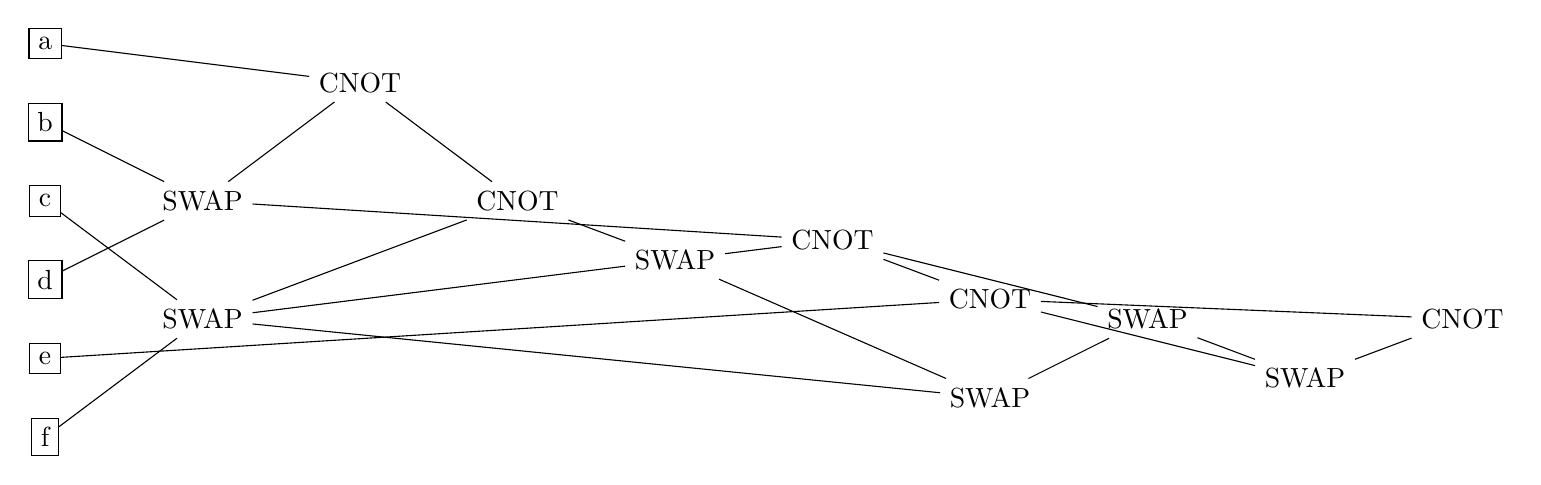
\begin{tikzpicture}
    
    \node [draw, rectangle] (a) at (0,5) {a};
    \node [draw, rectangle] (b) at (0,4) {b};
    \node [draw, rectangle] (c) at (0,3) {c};
    \node [draw, rectangle] (d) at (0,2) {d};
    \node [draw, rectangle] (e) at (0,1) {e};
    \node [draw, rectangle] (f) at (0,0) {f};
    
    \node (swap1) at (2,3) {SWAP};
    \node (swap2) at (2,1.5) {SWAP};
    \node (cnot1) at (4,4.5) {CNOT};
    \node (cnot2) at (6,3) {CNOT};
    \node (swap3) at (8,2.25) {SWAP};
    \node (cnot3) at (10,2.5) {CNOT};
    \node (cnot4) at (12,1.75) {CNOT};
    \node (swap4) at (12,0.5) {SWAP};
    \node (swap5) at (14,1.5) {SWAP};
    \node (swap6) at (16,0.75) {SWAP};
    \node (cnot5) at (18,1.5) {CNOT};
    
    \draw (b) -- (swap1);
    \draw (d) -- (swap1);
    
    \draw (c) -- (swap2);
    \draw (f) -- (swap2);
    
    \draw (a) -- (cnot1);
    \draw (swap1) -- (cnot1);
    
    \draw (cnot1) -- (cnot2);
    \draw (swap2) -- (cnot2);
    
    \draw (cnot2) -- (swap3);
    \draw (swap2) -- (swap3);
    
    \draw (swap1) -- (cnot3);
    \draw (swap3) -- (cnot3);
    
    \draw (cnot3) -- (cnot4);
    \draw (e) -- (cnot4);
    
    \draw (swap2) -- (swap4);
    \draw (swap3) -- (swap4);
    
    \draw (cnot3) -- (swap5);
    \draw (swap4) -- (swap5);
    
    \draw (cnot4) -- (swap6);
    \draw (swap5) -- (swap6);
    
    \draw (swap6) -- (cnot5);
    \draw (cnot4) -- (cnot5);
    
\end{tikzpicture}
}
Latency: $1440 + 400 = 1840$ ns

}
\label{fig:map_ex_depend_resch}

\label{fig:map_ex_routing}
\caption{Naive initial placement after routing}
\end{figure}
[\ldots{}]
In this case, we can apply scheduling, indeed. The first result with an optimal routing and scheduling would be this one.
Note that the circuit complexity has grown and, thus, the amount of possible errors along the circuit.
Remember that Quantum gates are well known to be highly faulty.


\begin{figure}
\centering
\subfigure[Routed circuit re-scheduled]{

\resizebox{.5\textwidth}{!}{
    \Qcircuit @C=.5em @R=.7em {
 \lstick{a \to Q_0} & \qw & \qw & \qw & \qw & \targ & \qw & \qw & \qw & \qw & \qw & \qw & \qw & \qw & \qw & \qw & \qw & \qw & \qw\\
\lstick{b \to Q_1} & \qswap & \push{d} \qw & \qw & \qw & \qw & \qw & \qw & \qw & \ctrl{2} & \targ & \qw & \qw & \qw & \qw & \qswap & \push{f} \qw & \targ & \qw\\
\lstick{c \to Q_2} & \qw & \qw & \qswap & \push{f} \qw & \qw & \qw & \qw & \qw & \qw & \qw & \qswap & \push{b} \qw & \qw & \qw & \qw & \qw & \qw & \qw\\
\lstick{d \to Q_3} & \qswap \qwx[-2] & \push{b} \qw & \qw & \qw & \ctrl{-3} & \targ & \qswap & \push{c} \qw & \targ & \qw & \qw & \qw & \qswap & \push{f} \qw & \qswap \qwx[-2] & \push{d} \qw & \qw & \qw\\
\lstick{e \to Q_4} & \qw & \qw & \qw & \qw & \qw & \qw & \qw & \qw & \qw & \ctrl{-3} & \qw & \qw & \qw & \qw & \qw & \qw & \ctrl{-3} & \qw\\
\lstick{f \to Q_5} & \qw & \qw & \qswap \qwx[-3] & \push{c} \qw & \qw & \ctrl{-2} & \qswap \qwx[-2] & \push{b} \qw & \qw & \qw & \qswap \qwx[-3] & \push{f} \qw & \qswap \qwx[-2] & \push{c} \qw & \qw & \qw & \qw & \qw \gategroup{1}{2}{6}{5}{.7em}{--} \gategroup{1}{6}{6}{6}{.7em}{--} \gategroup{1}{7}{6}{7}{.7em}{--} \gategroup{1}{8}{6}{9}{.7em}{--} \gategroup{1}{10}{6}{10}{.7em}{--} \gategroup{1}{11}{6}{13}{.7em}{--} \gategroup{1}{14}{6}{15}{.7em}{--} \gategroup{1}{16}{6}{17}{.7em}{--} \gategroup{1}{18}{6}{18}{.7em}{--}
 }
}

}
\label{fig:map_ex_circ_resch}

\subfigure[Dependence graph after re-scheduling]{
\resizebox{.75\textwidth}{!}{%
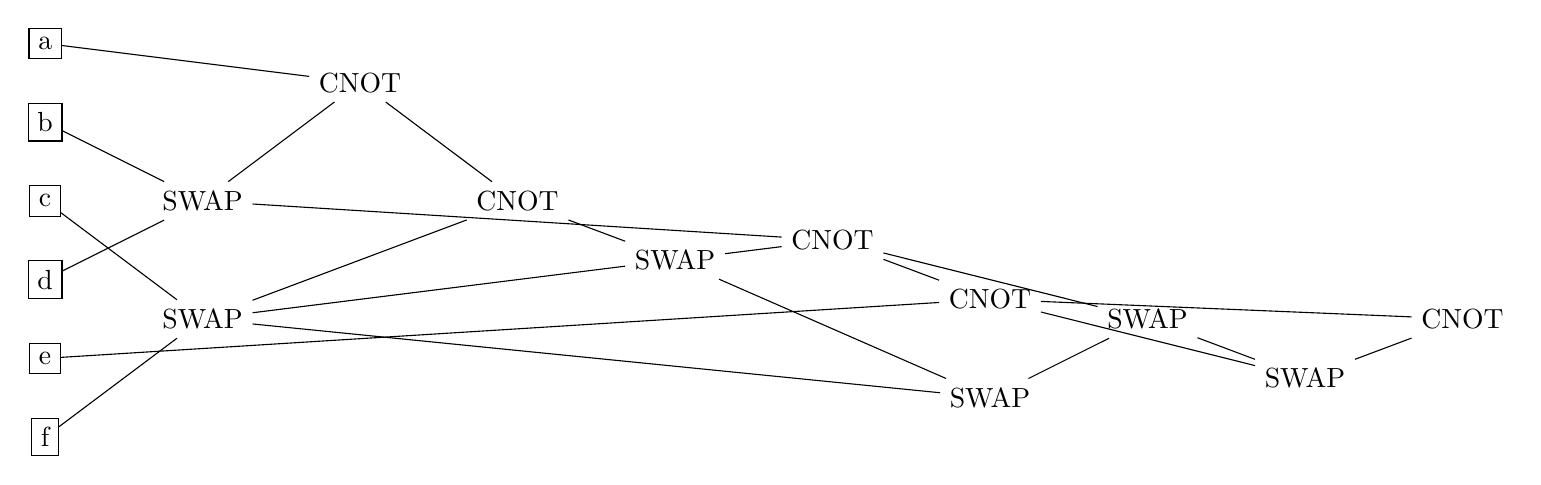
\begin{tikzpicture}
    
    \node [draw, rectangle] (a) at (0,5) {a};
    \node [draw, rectangle] (b) at (0,4) {b};
    \node [draw, rectangle] (c) at (0,3) {c};
    \node [draw, rectangle] (d) at (0,2) {d};
    \node [draw, rectangle] (e) at (0,1) {e};
    \node [draw, rectangle] (f) at (0,0) {f};
    
    \node (swap1) at (2,3) {SWAP};
    \node (swap2) at (2,1.5) {SWAP};
    \node (cnot1) at (4,4.5) {CNOT};
    \node (cnot2) at (6,3) {CNOT};
    \node (swap3) at (8,2.25) {SWAP};
    \node (cnot3) at (10,2.5) {CNOT};
    \node (cnot4) at (12,1.75) {CNOT};
    \node (swap4) at (12,0.5) {SWAP};
    \node (swap5) at (14,1.5) {SWAP};
    \node (swap6) at (16,0.75) {SWAP};
    \node (cnot5) at (18,1.5) {CNOT};
    
    \draw (b) -- (swap1);
    \draw (d) -- (swap1);
    
    \draw (c) -- (swap2);
    \draw (f) -- (swap2);
    
    \draw (a) -- (cnot1);
    \draw (swap1) -- (cnot1);
    
    \draw (cnot1) -- (cnot2);
    \draw (swap2) -- (cnot2);
    
    \draw (cnot2) -- (swap3);
    \draw (swap2) -- (swap3);
    
    \draw (swap1) -- (cnot3);
    \draw (swap3) -- (cnot3);
    
    \draw (cnot3) -- (cnot4);
    \draw (e) -- (cnot4);
    
    \draw (swap2) -- (swap4);
    \draw (swap3) -- (swap4);
    
    \draw (cnot3) -- (swap5);
    \draw (swap4) -- (swap5);
    
    \draw (cnot4) -- (swap6);
    \draw (swap5) -- (swap6);
    
    \draw (swap6) -- (cnot5);
    \draw (cnot4) -- (cnot5);
    
\end{tikzpicture}
}
Latency: 1520 ns
      
}
\label{fig:map_ex_depend_resch}

\label{fig:map_ex_resch}
\caption{Naive initial placement routed and re-scheduled}
\end{figure}
With an optimized initial placement, or a real optimized mapping the circuit could be the  same without adding any gate.
No routing is required.



\begin{figure}
\centering
\subfigure[Optimal initiapl placement]{
%\resizebox{.3\textwidth}{!}{
     \Qcircuit @C=1em @R=.7em {
     \lstick{a \to Q_0} & \targ & \qw & \qw & \qw & \qw & \qw\\
\lstick{b \to Q_2} & \ctrl{-1} & \targ & \qw & \qw & \qw & \qw\\
\lstick{c \to Q_5} & \qw & \ctrl{-1} & \targ & \qw & \qw & \qw\\
\lstick{d \to Q_3} & \qw & \qw & \ctrl{-1} & \targ & \qw & \qw\\
\lstick{e \to Q_1} & \qw & \qw & \qw & \ctrl{-1} & \targ & \qw\\
\lstick{f \to Q_4} & \qw & \qw & \qw & \qw & \ctrl{-1} & \qw
}
%}
}
\label{fig:map_ex_circ_optim}

\subfigure[Chip layout with the qubits with optimal initial placement]{
     \resizebox{0.45\textwidth}{!}{%
     \begin{tikzpicture}[x=5mm,y=5mm]
 % \tikzstyle{every node} = [circle, fill=gray!30]
 % \node [green] at (0,0) {[circle, fill=gray!30]};
 \draw node[fill=cyan,circle,minimum size=0.3cm] at (0,0) {};
 % \node [cyan] at (10,0) {\textbullet};
 \draw node[fill=cyan,circle,minimum size=0.3cm] at (10,0) {};
 % \node [green] at (20,0) {\textbullet};
 \draw node[fill=cyan,circle,minimum size=0.3cm] at (20,0) {};
 % \node [red] at (5,5) {\textbullet};
 \draw node[fill=cyan,circle,minimum size=0.3cm] at (5,5) {};
 % \node [red] at (5,-5) {\textbullet};
 \draw node[fill=cyan,circle,minimum size=0.3cm] at (5,-5) {};
 % \node [red] at (15,5) {\textbullet};
 \draw node[fill=cyan,circle,minimum size=0.3cm] at (15,5) {};
 % \node [red] at (15,-5) {\textbullet};
 \draw node[fill=cyan,circle,minimum size=0.3cm] at (15,-5) {};

 \node [purple] at (2,0) {\textbf{b} $\to$ \textbf{2}};
 \node [purple] at (12,0) {\textbf{d} $\to$ \textbf{3}};
 \node [purple] at (22,0) {\textbf{f} $\to$ \textbf{4}};
 \node [purple] at (7,5) {\textbf{a} $\to$ \textbf{0}};
 \node [purple] at (7,-5) {\textbf{c} $\to$ \textbf{5}};
 \node [purple] at (17,5) {\textbf{e} $\to$ \textbf{1}};
 \node [purple] at (17,-5) {\textbf{6}};

 % \draw[{Circle[red]}-Latex] (0,0) -- (2,0);
 \draw[-Latex] (0.1, 0.4)  -- (4.6,4.9)   node [midway, above, sloped] {0};
 \draw[-Latex] (4.8,4.7)   -- (0.3,0.2)  node [midway, below, sloped] {8};

 \draw[-Latex] (5.4, 4.9)   -- (9.9,0.4)  node [midway, above, sloped] {1};
 \draw[-Latex] (9.7,0.2) -- (5.2,4.7)   node [midway, below, sloped] {9};

 \draw[-Latex] (10.1,0.4)  -- (14.6,4.9)  node [midway, above, sloped] {2};
 \draw[-Latex] (14.8,4.7)  -- (10.3,0.2) node [midway, below, sloped] {10};

 \draw[-Latex] (15.4, 4.9)  -- (19.9,0.4)  node [midway, above, sloped] {3};
 \draw[-Latex] (19.7,0.2) -- (15.2,4.7)  node [midway, below, sloped] {11};

 \draw[-Latex] (0.4,-0.1) -- (4.9,-4.6)  node [midway, above, sloped] {4};
 \draw[-Latex] (4.7,-4.8) -- (0.2,-0.3)  node [midway, below, sloped] {12};

 \draw[-Latex] (5.1, -4.6) -- (9.6,-0.1) node [midway, above, sloped] {5};
 \draw[-Latex] (9.8, -0.3) -- (5.3, -4.8) node [midway, below, sloped] {13};

 \draw[-Latex] (10.4,-0.1) -- (14.9,-4.6) node [midway, above, sloped] {6};
 \draw[-Latex] (14.7,-4.8) -- (10.2,-0.3) node [midway, below, sloped] {14};

 \draw[-Latex] (15.1,-4.6) -- (19.6,-0.1) node [midway, above, sloped] {7};
 \draw[-Latex] (19.8,-0.3)  -- (15.3,-4.8) node [midway, below, sloped] {15};


 \end{tikzpicture}
 }
}
\label{fig:map_ex_chip_optim}

\label{fig:optimal_init_place}
\caption{Optimal initial placement}
\end{figure}


\begin{table}[htbp]
\caption{\label{tab:org9cd562c}
Difference between the naive initial placement and the optimal one in terms of number of operations and latency}
\centering
\begin{tabular}{ccc}
\hline
 & Optimal approach & Naive apprach\\
\hline
\# operations & 5 & 11\\
latency & 400 ns & 1520 ns\\
\hline
\end{tabular}
\end{table}
\end{itemize}

\section*{State of the art}
\label{sec:org9a5d195}

Quantum algorithms are meant to leverage the promising power of quantum computers \cite{coles18:quant_algor_implem_begin}.
Commonly described as quantum circuits, quantum algorithms are hardware agnostic.
Due to the variety of technologies that emerged with diverse specifications, there is a vast amount of literature on the algorithms -- high abstraction level --, neglecting hardware constraints.
From ion traps [? paper on ion traps] to superconducting qubits \cite{Barends_2014,Versluis_2017}, through quantum dots \cite{Hill_2015,Li_2018}, each layout has its own requirements and constraints.
Although all of them are arranged in a 2D -- planar -- structure, ion traps technologies are capable to connect the qubits in all-to-all networks while superconducting technologies connections form a grid shaped network where each qubit is connected to a maximum of four neighbors.
This grid behaviour establishes one of the main connectivity limitation in today's quantum chips, the NN constraint.
Also industry's superconducting chip layouts from IBM \cite{IBM_QX}, Google \cite{boixo16:charac_quant_suprem_near_term_devic} and Rigetti \cite{Sete_2016} follow this structural limitations.

As for the high abstraction level of the quantum algorithm, a link between the algorithms and the devices is required \cite{Fu_2016}.
As in classical computation, the algorithms should go through a compilation process in order to adapt them to the hosting device.
Certainly, the mapping procedure is an important element of this process based on three sub-tasks: scheduling, initial placement and routing; as we considered before.

There is a considerable amount of literature on the mapping task.
Initial works on this field \cite{Metodi_2006,Whitney_2007,Bahreini_2015} focused primarily on the definition of what they characterized as a \emph{scheduler} able to parallelize operations and add the required gates to route qubits.
They would consider general connectivity constraints as the NN one, common for most of the devices -- although the works were examining ion-traps as hardware implementations.
The proposed techniques by these works examine a dependency graph looking for the best way to organize qubits and operations.
The majority of the methods use latency as the metric to minimize, however some of them \cite{Farghadan_2017} would minimize in number of SWAP operations.
As it will be explained in the next section, to minimize in latency stands for time optimization while minimize in number of SWAP operations means to find the minimal number of operations required.
Following a similar reasoning as the first approaches, more complex solutions \cite{booth18:compar_integ_const_progr_tempor} have been published using Constraint Programming together with temporal planning, optimizing in latency as well.
Also, several publications \cite{Lye_2015,Wille_2016} outline only the routing sub-task using the number of SWAPS as the metric to minimize.

A recent review of the literature on the mapping topic focused on device specific mapping algorithms, with promising results.
In all the cases, taking into account the specific chip connectivity constrain.
IBM's chip have been gaining much attention due to the open online tools that make the chips accessible to everybody.
Various approaches to mapping algorithms for the IBM family of chips have been proposed \cite{zulehner17:effic_method_mappin_quant_circuit,Siraichi_2018,mckay18:qiskit_backen_specif_openq_openp_exper,Dueck_2018}.
Zulehner et. al \cite{zulehner17:effic_method_mappin_quant_circuit} developed a routing algorithm that optimizes in the number of SWAPs building a graph -- similarly to previous works --  and searching the best route in the chip layout with the A* algorithm.
Siraichi et. al \cite{Siraichi_2018} work defines a weighted dependence graph where the mapping algorithm is able to find a solution for all the mapping steps, initial placement, scheduling and routing.
Also, apart from the works related to the IBM devices, Rigetti's devices have been approached \cite{Venturelli_2018}.

Many attempts have been made \cite{Dousti_2014,Heckey_2015,hwang18:hierar_system_mappin_large_scale,murphy18:contr,Lao_2018} with the purpose of develop a FT mapping able to work at the logical -- qubit -- level.
However, due to the high complexity of the QEC techniques, quantum chips with large amounts of qubits are still theory.
More recent evidence \cite{Preskill_2018}, proposes the Noisy Intermediate-Scale Quantum (NISQ) devices as the next step for near future hardware with an amount of 50-100 qubits and without QEC or much simpler encodings.
Several studies, for instance \cite{tannu18:case_variab_aware_polic_nisq,paler18:nisq,paler18:influen_initial_qubit_placem_durin}, have been conducted on the mapping algorithms required for NISQ devices.
Also, the works on device specific solutions \cite{zulehner17:effic_method_mappin_quant_circuit,Siraichi_2018,mckay18:qiskit_backen_specif_openq_openp_exper,Dueck_2018,Venturelli_2018} described before, could be considered part of the NISQ works collection.
Although they do not approach the NISQ problem in general, it is true that the devices they tackle are NISQ devices, they have low number of qubits and high error rates.

Besides latency and the number of operations that serve to feedback the quality of a mapping algorithm, few studies have been published on quantum metrics.
Although widely investigated, there are not too many quantum metrics.
Fidelity has been addressed in order to characterize the error of a quantum circuit based on the qubits state \cite{Jozsa_1994,Nielsen_2009}.
And, recently, Quantum Volume has been defined to assert the capability of a quantum computer \cite{Moll_2018}.
In the next section and in \href{chapter-3.org}{Metrics} we offer an overview of the important metrics in this work.

\section*{Mapping metrics}
\label{sec:org767d700}

As outlined in the state of the art, the literature considers mainly two metrics to optimize in their mapping algorithms, the added \textbf{latency} and the \textbf{number} of introduced \textbf{operations} after the mapping procedure.
The routing step from the mapping process introduces SWAP gates in the quantum circuit in order to move the qubits around in the layout.
And latency is the time required to run a quantum circuit in a given quantum device.
It depends on the chip cycle time and the \textbf{depth} of the circuit, that is the number of cycles the algorithm encloses.
Actually, most of the studies [REFERENCES] assert the latency in terms of circuit depth, avoiding the cycle time specification of any device.
E.g. in Fig. \ref{fig:latency_swaps_ex}, one can see how after some mapping process some SWAP operations have been added as well as the depth of the circuit or latency grows.
From five cycles depth in the original circuit to nine cycles.


\begin{figure}
    \centering

\subfigure[Gray encoder quantum circuit]{

\resizebox{0.3\textwidth}{!}{
   \Qcircuit @C=1em @R=.7em {
\lstick{a} & \targ & \qw & \qw & \qw & \qw & \qw\\
\lstick{b} & \ctrl{-1} & \targ & \qw & \qw & \qw & \qw\\
\lstick{c} & \qw & \ctrl{-1} & \targ & \qw & \qw & \qw\\
\lstick{d} & \qw & \qw & \ctrl{-1} & \targ & \qw & \qw\\
\lstick{e} & \qw & \qw & \qw & \ctrl{-1} & \targ & \qw\\
\lstick{f} & \qw & \qw & \qw & \qw & \ctrl{-1} & \qw
}
}

}
\label{fig:latency_swaps_ex_orig}

\subfigure[Mapped Gray encoder for the SC-7 chip. Each circuit part surrounded by a dashed line is a cycle]{

\resizebox{0.4\textwidth}{!}{
    \Qcircuit @C=.5em @R=.7em {
 \lstick{a \to Q_0} & \qw & \qw & \qw & \qw & \targ & \qw & \qw & \qw & \qw & \qw & \qw & \qw & \qw & \qw & \qw & \qw & \qw & \qw\\
\lstick{b \to Q_1} & \qswap & \push{d} \qw & \qw & \qw & \qw & \qw & \qw & \qw & \ctrl{2} & \targ & \qw & \qw & \qw & \qw & \qswap & \push{f} \qw & \targ & \qw\\
\lstick{c \to Q_2} & \qw & \qw & \qswap & \push{f} \qw & \qw & \qw & \qw & \qw & \qw & \qw & \qswap & \push{b} \qw & \qw & \qw & \qw & \qw & \qw & \qw\\
\lstick{d \to Q_3} & \qswap \qwx[-2] & \push{b} \qw & \qw & \qw & \ctrl{-3} & \targ & \qswap & \push{c} \qw & \targ & \qw & \qw & \qw & \qswap & \push{f} \qw & \qswap \qwx[-2] & \push{d} \qw & \qw & \qw\\
\lstick{e \to Q_4} & \qw & \qw & \qw & \qw & \qw & \qw & \qw & \qw & \qw & \ctrl{-3} & \qw & \qw & \qw & \qw & \qw & \qw & \ctrl{-3} & \qw\\
\lstick{f \to Q_5} & \qw & \qw & \qswap \qwx[-3] & \push{c} \qw & \qw & \ctrl{-2} & \qswap \qwx[-2] & \push{b} \qw & \qw & \qw & \qswap \qwx[-3] & \push{f} \qw & \qswap \qwx[-2] & \push{c} \qw & \qw & \qw & \qw & \qw \gategroup{1}{2}{6}{5}{.7em}{--} \gategroup{1}{6}{6}{6}{.7em}{--} \gategroup{1}{7}{6}{7}{.7em}{--} \gategroup{1}{8}{6}{9}{.7em}{--} \gategroup{1}{10}{6}{10}{.7em}{--} \gategroup{1}{11}{6}{13}{.7em}{--} \gategroup{1}{14}{6}{15}{.7em}{--} \gategroup{1}{16}{6}{17}{.7em}{--} \gategroup{1}{18}{6}{18}{.7em}{--}
 }
}

}
\label{fig:latency_swaps_ex_map}

\caption{Circuit mapping example}
\label{fig:latency_swaps_ex}
\end{figure}

The ideal mapping would be the one affecting the least as possible the original circuit or, what is the same, introducing the least amount of errors.
Clearly, both, latency and number of SWAPs, are direct effects of the mapping procedure that have an impact in the error increase as well.
To optimize in any of them stands on correct -- but not sufficient -- reasoning.
Latency optimization deems that the leading error source comes from the qubit lifetime.
And, indeed, time is a main issue in quantum computing.
Decoherence time is not only a maximum qubit lifetime, it is harder and harder to hold a quantum state for use times closer to the decoherence time.
On the other hand, to optimize in number of SWAPs stands on the intuition that the gate error is the preeminent error in a quantum device.
Although intuitively one can think that the more operations are in a circuit, the longer it will be; as seen in the [PROBLEM STATEMENT SECTION], the higher the number of operations does not necessarily mean the longer circuit depth.
Several operations can be run in parallel in the same cycle -- at the same time.
Actually, to minimize in latency is to maximize in parallelism.
Therefore, even though related, to optimize in one or the other holds different baselines.

Nonetheless, these metrics are not enough to assert how good the mapping process is.
They are related with the error rate increase but the relationship is not totally clear.
For instance, it could be the case that concatenation of errors introduced by contiguous gates would end up in a correction of the first error.
Or, that the busier the qubit is, the less affected by decoherence would be.
Then, one question arises.
What would be the best metric?
Definitely, the optimal solution would be to optimize directly in terms of the error rate.
But, in order to do that, a precise prediction of the error should be done and this is a hard computational task in quantum computing.

So that we could do a proper assessment of mapping algorithms, in our research we analyzed these two metrics amongst other different ones as fidelity, probability of success or quantum volume and their relationship with the error generated after the mapping.
We will define these metrics in the \href{chapter-3.org}{Metrics} section.
